\documentclass[../../../../main.tex]{subfiles}
\begin{document}

\begin{flushright}
\footnotesize\textit{【自動文字起こし・要確認】}
\end{flushright}

[解] 4頂点 $O, A, B, C$ とし、点 $X$ に対し $\overrightarrow{OX} = \vec{x}$ とすると \\
$\vec{a}, \vec{b}, \vec{c}$ は一次独立 $\cdots \circledast$ である。題意から
\begin{align*}
\vec{a} \cdot (\vec{c} - \vec{b}) &= 0 \quad \cdots \text{②} \\
\vec{b} \cdot (\vec{a} - \vec{c}) &= 0 \quad \cdots \text{③} \\
\vec{c} \cdot (\vec{b} - \vec{a}) &= 0 \quad \cdots \text{④}
\end{align*}
$OX$ の中点 $X'$、四面体 $OABC$ の重心 $G$ ； $AB, BC, CA$ の中点 $P, Q, R$ として
\begin{align*}
\overrightarrow{GA'} &= \frac{1}{4} (\vec{a} - \vec{b} - \vec{c}) \\
\overrightarrow{GB'} &= \frac{1}{4} (-\vec{a} + \vec{b} - \vec{c}) \\
\overrightarrow{GC'} &= \frac{1}{4} (-\vec{a} - \vec{b} + \vec{c}) \\
\overrightarrow{GP} &= \frac{1}{4} (\vec{a} + \vec{b} - \vec{c}) \\
\overrightarrow{GQ} &= \frac{1}{4} (-\vec{a} + \vec{b} + \vec{c}) \\
\overrightarrow{GR} &= \frac{1}{4} (\vec{a} - \vec{b} + \vec{c})
\end{align*}
である。②〜④から
\[ \vec{a} \cdot \vec{c} = \vec{b} \cdot \vec{c} = \vec{a} \cdot \vec{b} \equiv A \]
だから $|\vec{a}|^2 + |\vec{b}|^2 + |\vec{c}|^2 = B$ とおけば、
\[ |\overrightarrow{GX'}|^2 = |\overrightarrow{GP}|^2 = |\overrightarrow{GQ}|^2 = |\overrightarrow{GR}|^2 = \frac{1}{16} (B - 2A) \quad (X' = A', B', C') \]
となり、たしかにこれらが $G$ を中心とする同一球面上にある。
\begin{center}
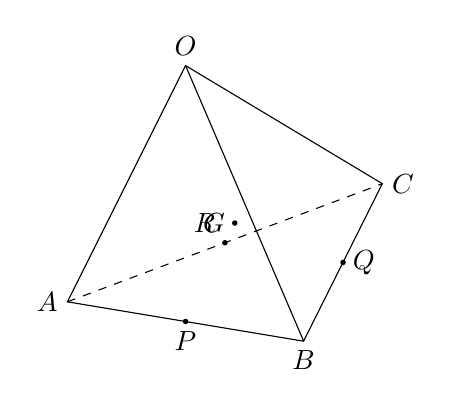
\begin{tikzpicture}
\coordinate (O) at (0,3);
\coordinate (A) at (-1.5,0);
\coordinate (B) at (1.5,-0.5);
\coordinate (C) at (2.5,1.5);
\draw (O) -- (A) -- (B) -- (C) -- (O);
\draw (O) -- (B);
\draw[dashed] (A) -- (C);
\node[above] at (O) {$O$};
\node[left] at (A) {$A$};
\node[below] at (B) {$B$};
\node[right] at (C) {$C$};
\coordinate (P) at (0,-0.25);
\coordinate (Q) at (2,0.5);
\coordinate (R) at (0.5,0.75);
\node[below] at (P) {$P$};
\node[right] at (Q) {$Q$};
\node[above left] at (R) {$R$};
\fill (P) circle (1pt);
\fill (Q) circle (1pt);
\fill (R) circle (1pt);
\coordinate (G) at (0.625, 1);
\node[left] at (G) {$G$};
\fill (G) circle (1pt);
\end{tikzpicture}
\end{center}

\end{document}
